\documentclass[11pt]{article}

\usepackage[utf8]{inputenc}
\usepackage[T1]{fontenc}
\usepackage{lmodern}
\usepackage{geometry}
\geometry{margin=1in}
\usepackage{amsmath,amssymb,amsfonts,amsthm,mathtools,bm}
\usepackage{physics}
\usepackage{tikz}
\usetikzlibrary{arrows.meta,positioning,calc,decorations.pathmorphing}
\usepackage{hyperref}
\usepackage{enumitem}
\usepackage{authblk}

\hypersetup{colorlinks=true,linkcolor=blue,citecolor=blue,urlcolor=blue}

\newtheorem{theorem}{Theorem}
\newtheorem{proposition}{Proposition}
\newtheorem{lemma}{Lemma}
\newtheorem{definition}{Definition}
\newtheorem{corollary}{Corollary}
\theoremstyle{remark}
\newtheorem{remark}{Remark}

\title{Frame-Dependent Photon Energy and Invariant Gravitational Collapse Criteria}
\author{Author Name}
\affil{Independent Research Draft}
\date{Draft \today}

\begin{document}
\maketitle

\begin{abstract}
Photon energy is not an observer-independent scalar: different inertial observers assign different frequencies and therefore different energies to the same null ray. This fact can tempt a misleading inference: if a sufficiently large boost can redshift a photon toward zero energy, or blueshift it without bound, then gravitational collapse of radiation might be observer-dependent. This paper introduces a clean separation between \emph{measured photon energy} and \emph{collapse-relevant invariants}. We formalize photon energy as the scalar measured by an observer four-velocity, $E_{(u)}=-p_\mu u^\mu$, while collapse criteria are encoded by invariant stress-energy localization, trapped surfaces, or center-of-momentum energy. The main result is a frame-invariance theorem: any collapse criterion expressible by a geometric condition on the spacetime, or by an invariant compactness functional of the total stress-energy, cannot be switched on or off by Lorentz boosting an observer. The proposed viewpoint is therefore not that photon energy is absolute, but that gravitational collapse is controlled by invariant organization of radiation rather than by any one observer's assigned frequency.
\end{abstract}

\tableofcontents

\section{Introduction}

The energy of a photon is commonly written as
\begin{equation}
E = h f = \hbar \omega .
\end{equation}
Since frequency is Doppler shifted, photon energy is frame-dependent. A receding observer can measure the photon as highly redshifted, while an approaching observer can measure it as highly blueshifted. At first glance this seems to create a paradox: if energy gravitates, and photon energy is relative, should black-hole formation from radiation also be relative?

This paper proposes a simple resolution. The quantity measured by an observer is relative; the existence of a trapped surface or black-hole region is geometric. Radiation may have frame-dependent local energy measurements, but collapse depends on invariant concentration of stress-energy. The same distinction appears in high-energy collision studies of black-hole formation, where apparent horizons and center-of-momentum invariants replace single-observer energy assignments.

\paragraph{New viewpoint.} The paper introduces a formal distinction between:
\begin{enumerate}[label=(\roman*)]
\item \textbf{frequency energy}: the observer-indexed scalar $E_{(u)}$;
\item \textbf{collapse energy}: invariant data of the full stress-energy distribution, such as Mandelstam $s$, quasi-local mass, compactness, or trapped-surface existence.
\end{enumerate}
The point is not to deny that photons gravitate. The point is that the gravitationally relevant question is not ``How energetic is the photon in my frame?'' but ``Is the full null stress-energy distribution invariantly compact enough to produce a trapped region?''

\section{Literature grounding}

Special relativity identifies the energy measured by an observer with a contraction of four-momentum and observer four-velocity. Relativistic Doppler shift gives the transformation of photon frequency under boosts. In general relativity, gravitational collapse is not defined by a coordinate-dependent energy label but by geometric structures such as trapped surfaces, apparent horizons, and event horizons. Classical high-energy collision work by Eardley and Giddings analyzes black-hole production through apparent-horizon construction rather than a single observer's photon frequency. Follow-up semiclassical analyses show that wavepacket localization and center-of-momentum energy are the relevant inputs.

This draft uses standard conventions with metric signature $(-,+,+,+)$ and units $c=1$ unless restored explicitly.

\section{Observer-measured photon energy}

\begin{definition}[Observer-measured photon energy]
Let $p^\mu$ be a future-directed null four-momentum, $p^2=0$, and let $u^\mu$ be a future-directed unit timelike observer four-velocity, $u^2=-1$. The energy measured by $u$ is
\begin{equation}
E_{(u)}(p) = - p_\mu u^\mu .
\end{equation}
\end{definition}

\begin{proposition}[Doppler scaling]
Let a photon propagate in the $+x$ direction with four-momentum $p^\mu=(\omega,\omega,0,0)$. Let $u^\mu=\gamma(1,v,0,0)$ be an observer moving in the same direction. Then
\begin{equation}
E_{(u)} = \gamma \omega (1-v)=\omega\sqrt{\frac{1-v}{1+v}} .
\end{equation}
As $v\to 1$, $E_{(u)}\to 0$.
\end{proposition}

\begin{proof}
With signature $(-,+,+,+)$,
\begin{equation}
E_{(u)}=-p\cdot u=-[-\gamma\omega+\gamma v\omega]=\gamma\omega(1-v).
\end{equation}
Using $\gamma=(1-v^2)^{-1/2}$ gives the final expression.
\end{proof}

\begin{remark}
No massive observer can reach $v=1$, and no photon rest frame exists. The limit $E_{(u)}\to0$ is a limiting sequence of observers, not a frame comoving with light.
\end{remark}


\begin{lemma}[Passive observer change versus active state change]
Let a physical null configuration be described by fixed tensor fields $(g,T)$ and momenta $p_i$. Replacing the observer $u$ by another future timelike unit vector $u'$ changes the measured scalars $E_{(u)}(p_i)$ but leaves every Lorentz scalar formed solely from the $p_i$ unchanged. By contrast, physically accelerating or otherwise preparing different incoming packets changes the state itself and may change its invariant collision data.
\end{lemma}

\begin{proof}
For a passive observer change the four-vectors $p_i$ are fixed geometric objects, so every contraction $p_i\cdot p_j$ is unchanged while $-p_i\cdot u$ changes because $u$ changes. For a common Lorentz transformation $\Lambda$ acting on all vectors,
\begin{equation}
 (\Lambda p_i)\cdot(\Lambda p_j)=p_i\cdot p_j.
\end{equation}
A physical preparation change is not a passive replacement of $u$ and is therefore not covered by this identity.
\end{proof}


\section{Invariant collision energy}

For one photon, $p^2=0$, so there is no rest energy or center-of-momentum frame. For two photons or two localized radiation packets, an invariant exists.

\begin{definition}[Two-packet invariant]
For two future-directed null momenta $p_1,p_2$, define
\begin{equation}
s=(p_1+p_2)^2=2p_1\cdot p_2 .
\end{equation}
With our signature, many particle-physics conventions use $s=-(p_1+p_2)^2$; here we track signs explicitly when needed. The invariant center-of-momentum energy is determined by $|s|^{1/2}$.
\end{definition}

For two photons of frequencies $\omega_1,\omega_2$ meeting at angle $\theta$,
\begin{equation}
E_{\rm cm}^2 = 2\omega_1\omega_2(1-\cos\theta),
\end{equation}
where the right-hand side is invariant under Lorentz transformations when the transformed frequencies and transformed angle are used together.

\begin{figure}[h]
\centering
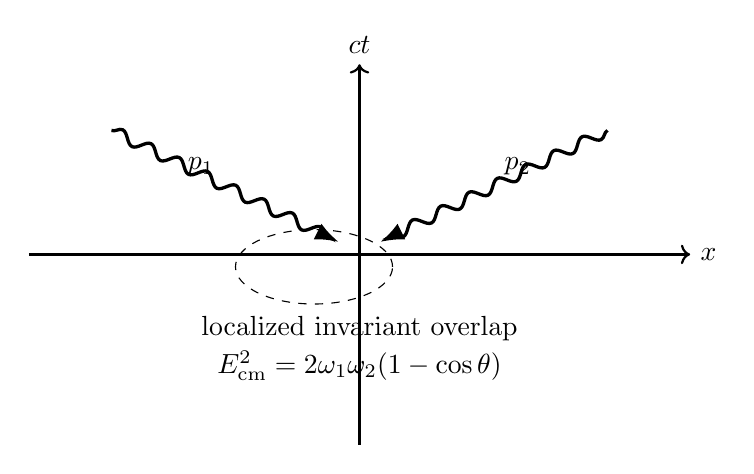
\begin{tikzpicture}[scale=1.05]
    \draw[->,thick] (-4,0) -- (4,0) node[right] {$x$};
    \draw[->,thick] (0,-2.3) -- (0,2.3) node[above] {$ct$};
    \draw[-{Latex[length=3mm]},very thick,decorate,decoration={snake,amplitude=0.7mm,segment length=4mm}] (-3,1.5) -- (-0.25,0.15) node[midway,above left] {$p_1$};
    \draw[-{Latex[length=3mm]},very thick,decorate,decoration={snake,amplitude=0.7mm,segment length=4mm}] (3,1.5) -- (0.25,0.15) node[midway,above right] {$p_2$};
    \draw[dashed] (-0.55,-0.15) ellipse (0.95 and 0.45);
    \node at (0,-0.9) {localized invariant overlap};
    \node at (0,-1.35) {$E_{\rm cm}^2=2\omega_1\omega_2(1-\cos\theta)$};
\end{tikzpicture}
\caption{A boost changes $\omega_1$, $\omega_2$, and the angle between rays, but not the invariant center-of-momentum data of the two-packet system.}
\end{figure}


\begin{proposition}[Exact head-on boost compensation]
Consider equal-energy head-on photons
\begin{equation}
 p_1=(E,E,0,0),\qquad p_2=(E,-E,0,0).
\end{equation}
Under a boost of rapidity $y$ in the $+x$ direction,
\begin{equation}
 E_1'=Ee^{-y},\qquad E_2'=Ee^{y}.
\end{equation}
Although one photon is arbitrarily redshifted and the other arbitrarily blueshifted as $|y|$ grows,
\begin{equation}
 E_1'E_2'=E^2,
 \qquad
 E_{\rm cm}^2=4E_1'E_2'=4E^2.
\end{equation}
Thus the divergent one-photon energies generated by the boost cancel exactly in the two-packet invariant.
\end{proposition}

\begin{proof}
The standard rapidity boost gives $p'^0=\cosh y\,p^0-\sinh y\,p^x$. Applying it to $p_1$ and $p_2$ gives $E e^{-y}$ and $E e^{y}$ respectively. Their product is $E^2$. Since the photons remain antiparallel, $1-\cos\theta'=2$, and therefore $E_{\rm cm}^2=2E_1'E_2'(2)=4E^2$.
\end{proof}


\section{Geometric collapse criteria}

\begin{definition}[Trapped surface]
A closed spacelike two-surface $S$ in a spacetime $(M,g)$ is future trapped if both future-directed null congruences orthogonal to $S$ have negative expansion:
\begin{equation}
\theta_+<0,\qquad \theta_-<0 .
\end{equation}
\end{definition}

This definition is geometric. It does not depend on a coordinate frame or on a chosen inertial observer.

\begin{definition}[Invariant compactness functional]
Let $\Omega$ be a spacelike compact region with characteristic areal radius $R(\Omega)$ and quasi-local energy $M(\Omega)$ defined covariantly, for example by Misner--Sharp mass in spherical symmetry or another quasi-local mass in appropriate settings. Define
\begin{equation}
\mathcal C(\Omega)=\frac{2G M(\Omega)}{R(\Omega)}.
\end{equation}
A compactness-based collapse condition has the schematic form $\mathcal C(\Omega)\gtrsim1$.
\end{definition}

The precise form of $M(\Omega)$ depends on symmetry and boundary conditions, but the key point is structural: a meaningful collapse criterion must be geometric or invariant, not the energy assigned by one observer to one ray.


\subsection{Center-of-momentum compactness and trappedness}
For an isolated localized radiation configuration with total four-momentum $P^\mu$ satisfying $P^2<0$, define the invariant center-of-momentum energy
\begin{equation}
 E_* = \sqrt{-P^2}.
\end{equation}
Let $\Sigma_*$ be the hypersurface orthogonal to $P^\mu$ and let $R_*$ be an areal or otherwise geometrically specified localization radius measured on $\Sigma_*$. A center-of-momentum compactness surrogate is
\begin{equation}
 \mathcal C_* = \frac{2GE_*}{R_*}
 \label{eq:com-compactness}
\end{equation}
when $c=1$. Both $E_*$ and a geometrically specified $R_*$ are independent of the observer used to decompose the same configuration. Equation~\eqref{eq:com-compactness} therefore isolates the two ingredients that a one-photon Doppler factor cannot supply: invariant total energy and invariant localization.

\begin{lemma}[Sign of null expansion is geometric]
Let $S$ be a spacelike two-surface and $k_\pm^\mu$ its future null normals normalized by $k_+\cdot k_-=-1$. Their expansions
\begin{equation}
 \theta_\pm=q^{\mu\nu}\nabla_\mu k^\pm_\nu
\end{equation}
are scalar functions on $S$ once the normalization is fixed. Hence the signs of $\theta_+$ and $\theta_-$, and therefore trappedness, cannot be changed by a passive Lorentz transformation of an observer tetrad.
\end{lemma}

\begin{proof}
The induced metric $q^{\mu\nu}$, the covariant derivative, and the null normals are geometric tensors. Their full contraction is a scalar. A passive change of coordinates or tetrad changes components but not the scalar value. A positive rescaling $k_+\mapsto e^f k_+$, $k_-\mapsto e^{-f}k_-$ preserves the sign of each expansion on a closed surface when the usual future orientation is retained.
\end{proof}

The Raychaudhuri equation provides the corresponding dynamical statement. For an affinely parameterized hypersurface-orthogonal null congruence,
\begin{equation}
 \frac{d\theta}{d\lambda}
 =-\frac12\theta^2-\sigma_{\mu\nu}\sigma^{\mu\nu}-R_{\mu\nu}k^\mu k^\nu.
 \label{eq:raychaudhuri-photon}
\end{equation}
Using Einstein's equation and $k^2=0$ gives
\begin{equation}
 R_{\mu\nu}k^\mu k^\nu
 =8\pi G\,T_{\mu\nu}k^\mu k^\nu.
\end{equation}
The focusing source is therefore a tensor contraction of the full stress-energy with the null tangent, not a selected observer's one-photon energy.


\section{Main theorem}

\begin{theorem}[Frame invariance of geometric collapse]
Let $(M,g,T)$ be a spacetime with stress-energy tensor $T_{\mu\nu}$. Let $\mathfrak C(M,g,T)$ be any collapse predicate satisfying:
\begin{enumerate}[label=(\alph*)]
\item \emph{diffeomorphism invariance}: if $(M,g,T)$ and $(M',g',T')$ are isometric as stress-energy-decorated spacetimes, then $\mathfrak C$ has the same truth value on both;
\item \emph{geometric definability}: $\mathfrak C$ is defined through trapped surfaces, curvature invariants, invariant quasi-local mass, or other tensorial/geometric data.
\end{enumerate}
Then changing the observer four-velocity $u^\mu$ used to assign photon energies $E_{(u)}=-p\cdot u$ cannot change the truth value of $\mathfrak C$.
\end{theorem}

\begin{proof}
A change of observer is a change in the timelike vector field used to decompose tensorial data into measured energy density, momentum density, and stress. It does not alter the underlying fields $(g,T)$. By hypothesis, $\mathfrak C$ is a function only of geometric/tensorial data and is invariant under isometries or coordinate changes. Therefore two observers may assign different local energies to the same null component, but they evaluate the same geometric structure. Hence $\mathfrak C$ is unchanged.
\end{proof}

\begin{corollary}[No boost loophole]
A Lorentz boost can redshift a photon arbitrarily close to zero energy for a sequence of receding massive observers, but it cannot remove an already-existing trapped surface. A Lorentz boost can also blueshift a photon without bound for a sequence of approaching observers, but it cannot create a trapped surface if no invariant compactness or trapped-surface condition is satisfied.
\end{corollary}

\section{Toy model: parallel versus head-on null beams}

Consider two ideal null beams with momenta $p_1$ and $p_2$.

\paragraph{Parallel limit.}
If $p_1\parallel p_2$, then $p_1\cdot p_2=0$ and the pair has vanishing invariant mass. Increasing the common lab-frame frequency does not by itself create a rest-frame energy for the system.

\paragraph{Head-on limit.}
If $p_1=(\omega,\omega,0,0)$ and $p_2=(\omega,-\omega,0,0)$, then
\begin{equation}
E_{\rm cm}=2\omega .
\end{equation}
A boost changes the two measured photon frequencies asymmetrically, but the product entering $E_{\rm cm}$ remains invariant.

\begin{proposition}[Angle-energy compensation]
For two photons, the combination $2\omega_1\omega_2(1-\cos\theta)$ is Lorentz invariant, although each factor separately changes under boosts.
\end{proposition}

\begin{proof}[Proof sketch]
The expression is the Lorentz scalar determined by the total four-momentum squared. Since $p_1\cdot p_2$ is invariant, the formula computed from frequencies and angle in any inertial frame gives the same scalar.
\end{proof}

\section{Discussion}

The proposed framing resolves the apparent conflict between relative photon energy and invariant gravitational collapse. Energy measured by an observer is real operational data, but it is not the whole gravitational criterion. In relativity, the stress-energy tensor is decomposed differently by different observers:
\begin{equation}
\rho_{(u)}=T_{\mu\nu}u^\mu u^\nu,
\end{equation}
while the tensor itself remains the object coupled to geometry. Thus, a single observer's decomposition cannot determine an observer-independent causal feature such as the presence of a trapped region.

The conceptual error is treating $E=hf$ as if it were an absolute gravitational charge. A better statement is:
\begin{quote}
Photon energy is observer-dependent; gravitational collapse is controlled by invariant localization of the total stress-energy distribution.
\end{quote}

\section{Conclusion}

This draft introduced a formal distinction between observer-measured photon energy and invariant collapse data. The main theorem shows that any geometric collapse criterion cannot be switched on or off by changing the observer. The result turns the original intuition into a precise negative theorem: frequency can be relative without making black-hole formation relative.

\begin{thebibliography}{9}

\bibitem{MTW}
C. W. Misner, K. S. Thorne, and J. A. Wheeler,
\textit{Gravitation}, W. H. Freeman, 1973.

\bibitem{Wald}
R. M. Wald,
\textit{General Relativity}, University of Chicago Press, 1984.

\bibitem{EardleyGiddings}
D. M. Eardley and S. B. Giddings,
``Classical black hole production in high-energy collisions,''
\textit{Physical Review D} \textbf{66}, 044011 (2002), arXiv:gr-qc/0201034.

\bibitem{GiddingsRychkov}
S. B. Giddings and V. S. Rychkov,
``Black holes from colliding wavepackets,''
\textit{Physical Review D} \textbf{70}, 104026 (2004), arXiv:hep-th/0409131.

\bibitem{HawkingEllis}
S. W. Hawking and G. F. R. Ellis,
\textit{The Large Scale Structure of Space-Time}, Cambridge University Press, 1973.

\bibitem{Carroll}
S. M. Carroll,
\textit{Spacetime and Geometry: An Introduction to General Relativity}, Addison-Wesley, 2004.

\end{thebibliography}

\end{document}
